%
% 01_Pitch_Detektion.tex
%
% (c) 2023 Florian Baumgartner, OST Ostschweizer Fachhochschule
%
% !TEX root = ../../buch.tex
% !TEX encoding = UTF-8
%
\section{Pitch-Detektion
\label{autotune:section:pitchDetektion}}
\rhead{Pitch-Detektion}
Bei einer einstimmigen Aufnahme, beispielsweise der menschlichen Stimme oder eines Blasinstruments,
wird die Grundharmonische als Tonhöhe angeschaut.
Es gilt nun, diese zu finden. Es gibt mehrere Möglichkeiten dies umzusetzen.
Im Rahmen dieses Papers werden zwei Methoden verglichen.

\subsection{Short-Time Fourier-Transformation (STFT)
\label{autotune:subsection:shortTimeFourierTransformation}}
Die Short-Time Fourier-Transformation (STFT) ist eine Fourier-Transformation, die auf einem kleinen,
zeitlich begrenzten Ausschnitt eines Signals angewendet wird.
Da es sich sich um einen diskreten Vorgang handelt, wird die STFT beschrieben als
\begin{equation}
    \mathbf{STFT}_x(m, w)
    =
    \sum_{n=-\infty}^{\infty}x(n)\;w(n-m)\;e^{-j\omega n}.
\end{equation}
Dabei definiert $x(n)$ das Signal, $w(n)$ das Fenster und $m$ den Verschiebungsparameter.
Üblicherweise wird ein Fenster der Länge $N$ verwendet, wobei $N$ eine Zweierpotenz ist.
Je länger das Zeitfenster, desto höher ist die physikalische Frequenzauflösung. Jedoch reduziert sich die zeitliche Spektrumabtastung.
Dieser Trade-Off kann gut anhand eines Beispiels gezeigt werden.

\[
    f_s = 44100\;\text{Samples/s} \quad\quad l_w = 23\;\text{ms} \quad\quad L = f_s \cdot l_w = 1014.3 \approx 1024\;\text{Samples}
\]
\[
    \Delta f = \frac{f_s}{L}\approx 43.07\;\text{Hz}
\]

Es fällt auf, dass mit einer Fensterlänge von 23\;ms die Frequenzauflösung bei nur 43.07\;Hz liegt.
Da einzelne Töne jedoch nur wenige Hertz auseinander liegen, können diese nur ungenau voneinander unterschieden werden.
Schnelle Melodien verhindern das Verlängern der Fensterzeit, da sonst mehrere Töne auf ein Segment fallen und nicht mehr identifiziert werden können.

Bei einer Fensterlänge von 23\;ms wird das Spektrum also ca. 43 mal pro Sekunde abgetastet.
Wie in Abbildung \ref{autotune:fig:pitchDetektionSTFT} zu sehen ist, können somit auch schnelle Tonhöhenänderung erkannt werden.

\begin{figure}
	\centering
	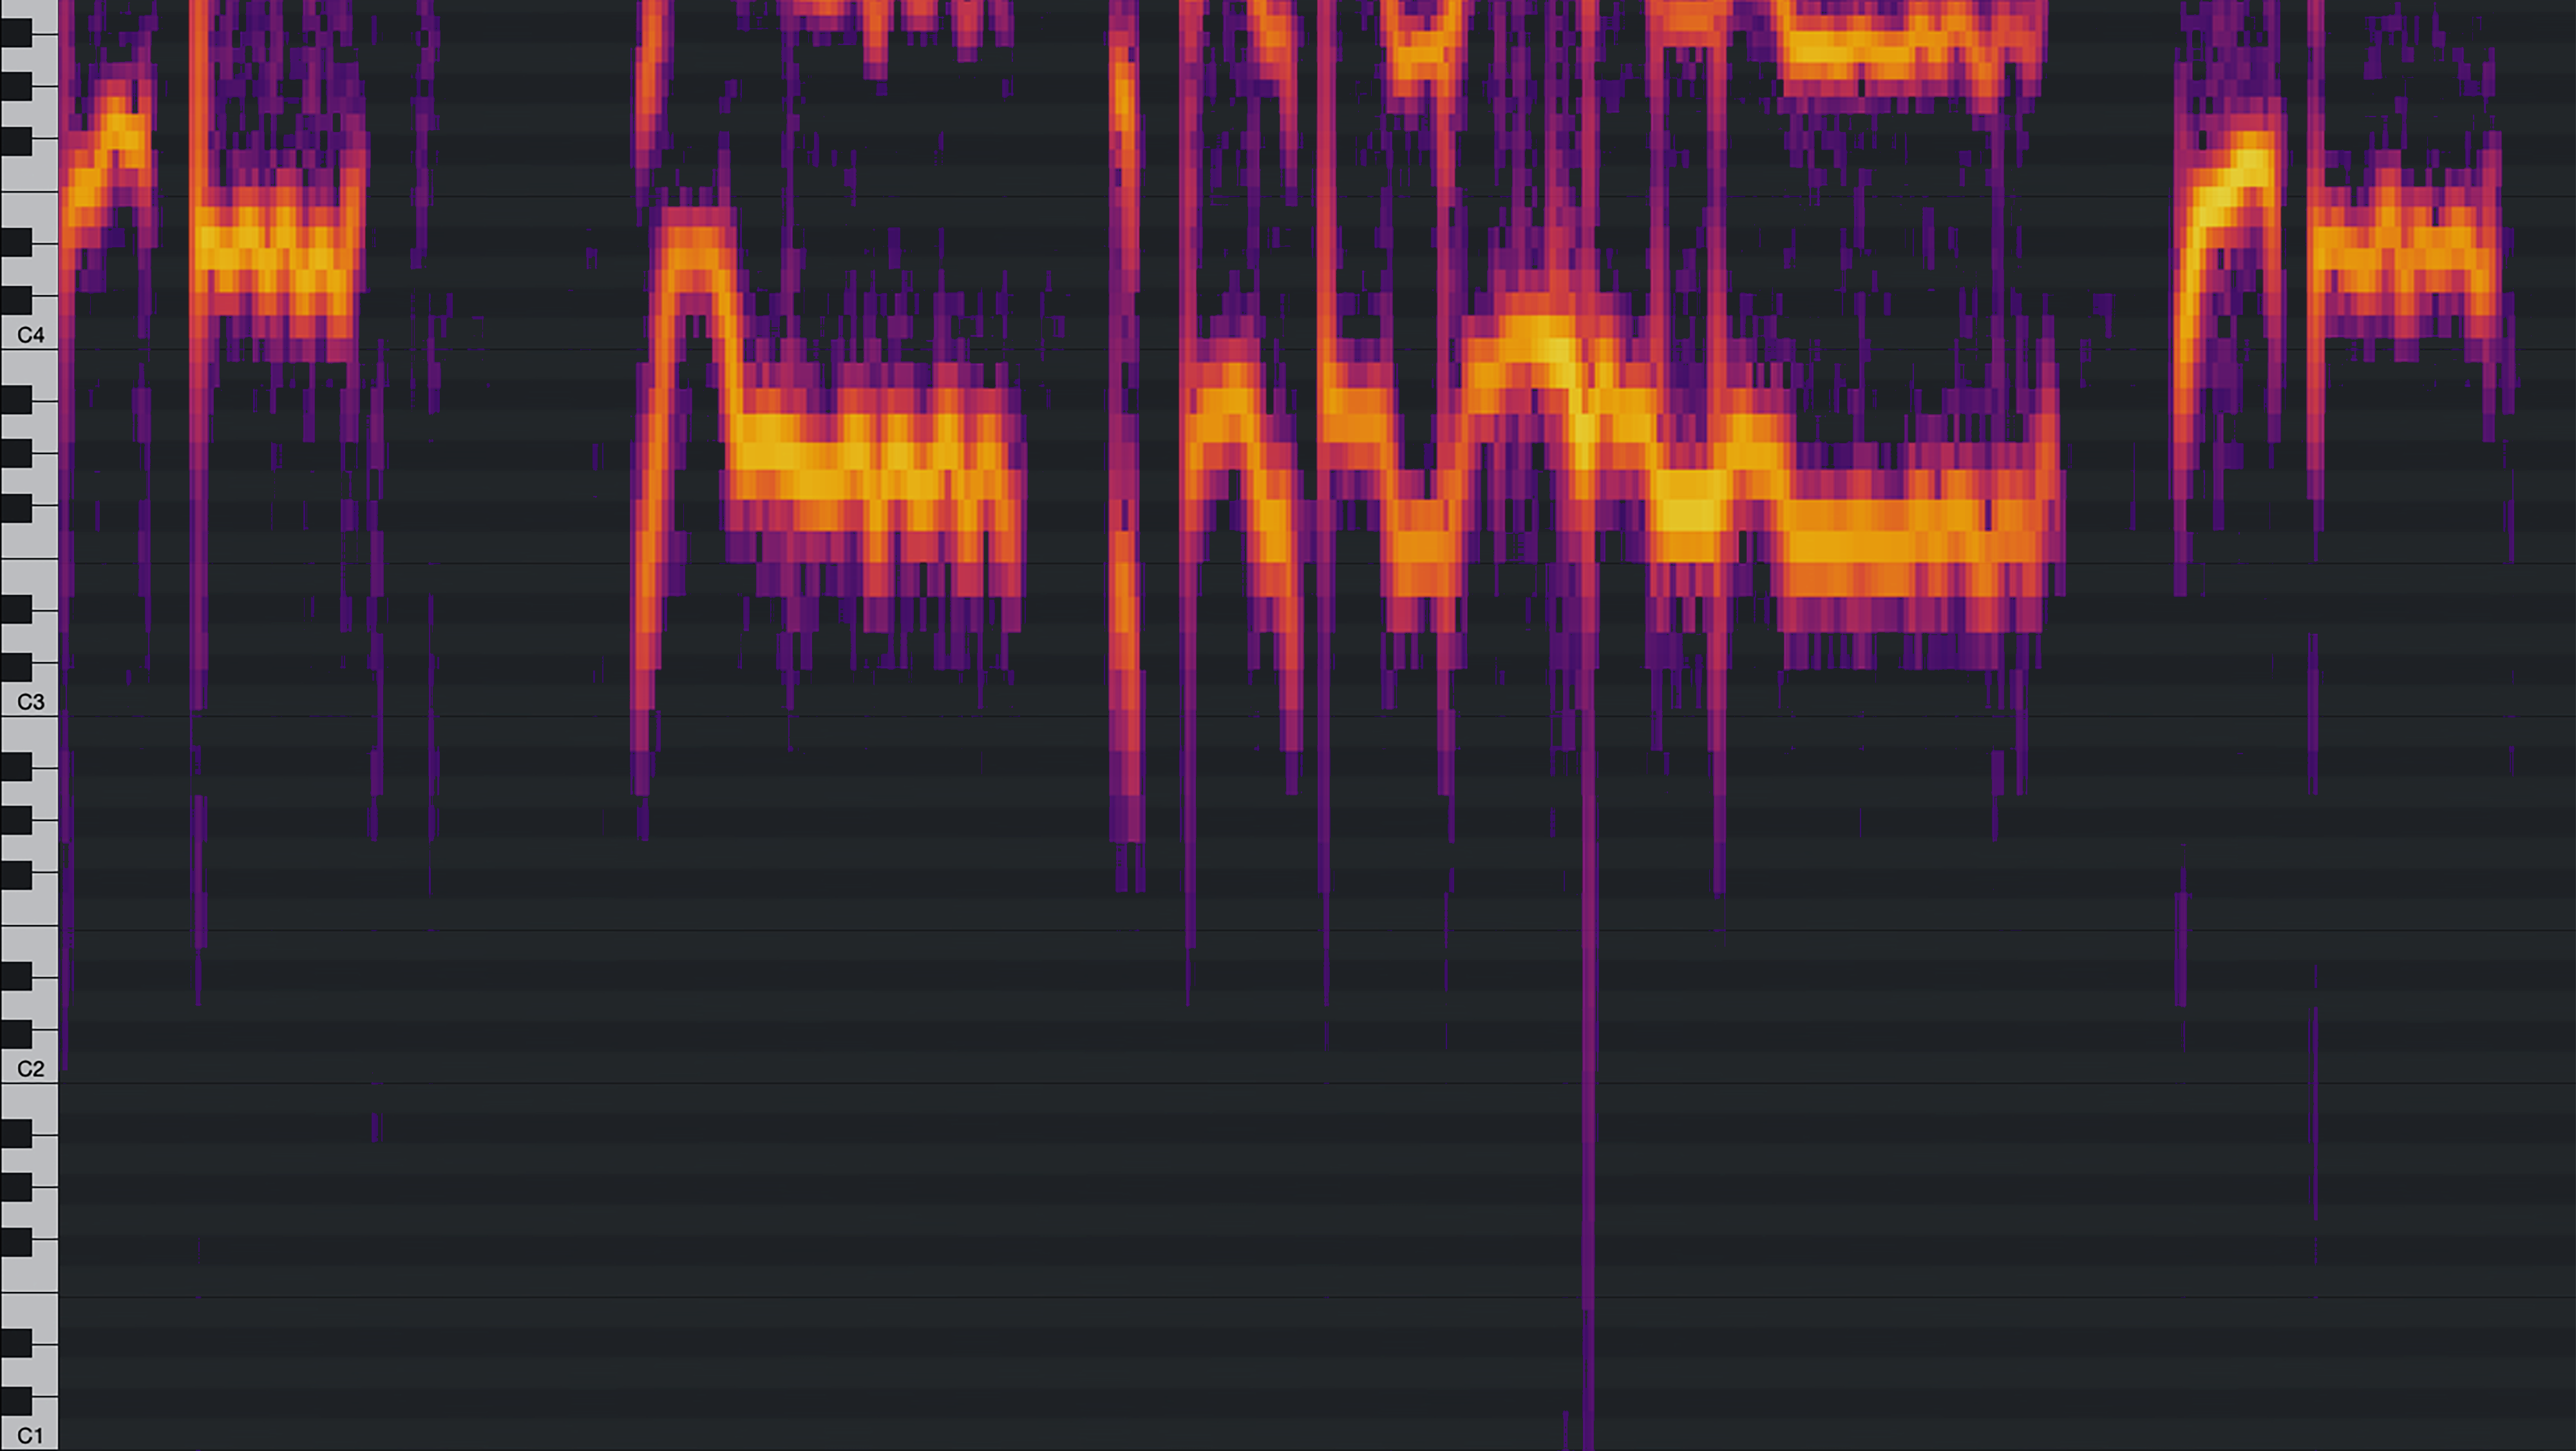
\includegraphics[width=\textwidth]{papers/autotune/images/Pianoscale_Example_Detuned_STFT.png}
	\caption{Pitch-Detektion mit STFT (Fensterlänge von 23\;ms).}
    \label{autotune:fig:pitchDetektionSTFT}
\end{figure}

Diese spektrale Darstellungsweise wird auch als Sonogramm bezeichnet. Mehr dazu im Kapitel \ref{chapter:sonogramm}.


Das konkrete bestimmen der Tonhöhe innerhalb eines Fensters kann auf verschiedene Arten umgesetzt werden.
Eine Möglichkeit ist das Bestimmen der Grundharmonischen durch das Finden des Maximums im Spektrum (Peak-Detektor).
Mathematisch ausgedrückt als

\begin{equation}
    f_{\text{pitch}}
    =
    \arg\max_{f}{\left | \; \mathbf{STFT}_x(m, w) \; \right |}^2.
\end{equation}


\subsection{Cumulative Mean Normalized Difference Function (CMNDF)
\label{autotune:subsection:cumultativeMeanNormalizedDifferenceFunction}}
Eine weitere Methode zur Tonhöhenbestimmung ist die Cumulative Mean Normalized Difference Function (CMNDF).
Diese Methode basiert auf der Auto-Korrelation des Signals welche definiert ist als

\begin{equation}
    \mathbf{ACF}(\tau, t)
    =
    \sum_{i=t}^{t+W}f(x_i)\cdot f(x_i+\tau).
\end{equation}

Dabei ist $\tau$ die Verzögerung innerhalb des Fensters und $W$ die Fensterlänge.
Daraus folgend kann die Quadrierte Differenz Funktion $\mathbf{DF}$ hergeleitet werden als

\begin{equation}
    \begin{aligned}
        \mathbf{DF}(\tau,t)
        &= \sum_{i=t}^{t+W}\left(f(x_i)-f(x_i+\tau)\right)^2 \\
        &= \sum_{i=t}^{t+W}\left(f(x_i)^2+f(x_i+\tau)^2-2 \cdot f(x_i) \cdot f(x_i + \tau)\right) \\
        &= \mathbf{ACF}(0,t)+\mathbf{ACF}(0,t+\tau)-2\cdot \mathbf{ACF}(\tau,t).
    \end{aligned}
\end{equation}

Die $\mathbf{DF}$ liefert den normalisierten absoluten \glqq Überlagerungsfehler\grqq\ zum Zeitpunkt $t$ des Signals $f$ und einer um $\tau$ verzögerten Version von $f$.
Bei $\tau=0$ ist der Überlagerungsfehler 0, da das Signal mit sich selbst verglichen wird.
Die $\mathbf{CMNDF}$ ist definiert als 

\begin{equation}
    \mathbf{CMNDF}(\tau,t)
    =
    \left\{
        \;\begin{array}{ll} 0 & \tau=0 \\
        \tau \cdot \frac{\mathbf{DF}(\tau,t)}{\sum\nolimits_{j=1}^{\tau} \mathbf{DF}(j,t)} & \tau > 0 \end{array}
    \right\}.
\end{equation}


Gesucht wird nun das erste lokale Minimum der CMNDF.
Dieses Minimum entspricht der Periodendauer der Grundharmonischen.
Grafisch dargestellt ist dies in Abbildung \ref{autotune:fig:cmndfMinimum}.

\begin{figure}
	\centering
	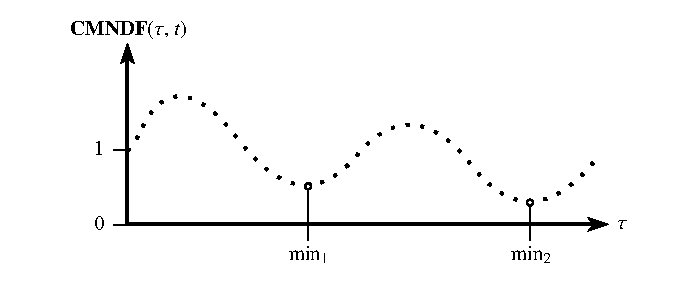
\includegraphics[width=0.8\textwidth]{papers/autotune/images/CMNDF_Minimum.pdf}
	\caption{Finden der lokalen Minima von CMNDF.}
    \label{autotune:fig:cmndfMinimum}
\end{figure}


Es fällt auf, dass die CMNDF mehrere lokale Minima aufweist.
Diese entsprechen den höhren Harmonischen und sind nicht von Interesse.
In der Praxis erweist es sich zum Teil als schwierig, das erste lokale Minimum zu finden.
Oft wird deshalb ein Schwellwert definiert.
An der Stelle wo die CMNDF diesen Schwellwert unterschreitet, wird das Minimum definiert.
Die Tonhöhe kann nun bestimmt werden als

\begin{equation}
    f_{pitch}
    =
    \frac{1}{min_1}.
\end{equation}


Die CMNDF ist im Vergleich zur STFT wesentlich effizienter und liefert sowohl eine hohe Frequenzauflösung als auch eine hohe zeitliche Auflösung.
Dies ist in Abbildung \ref{autotune:fig:pitchDetektionCMNDF} gut ersichtlich.

\begin{figure}
	\centering
	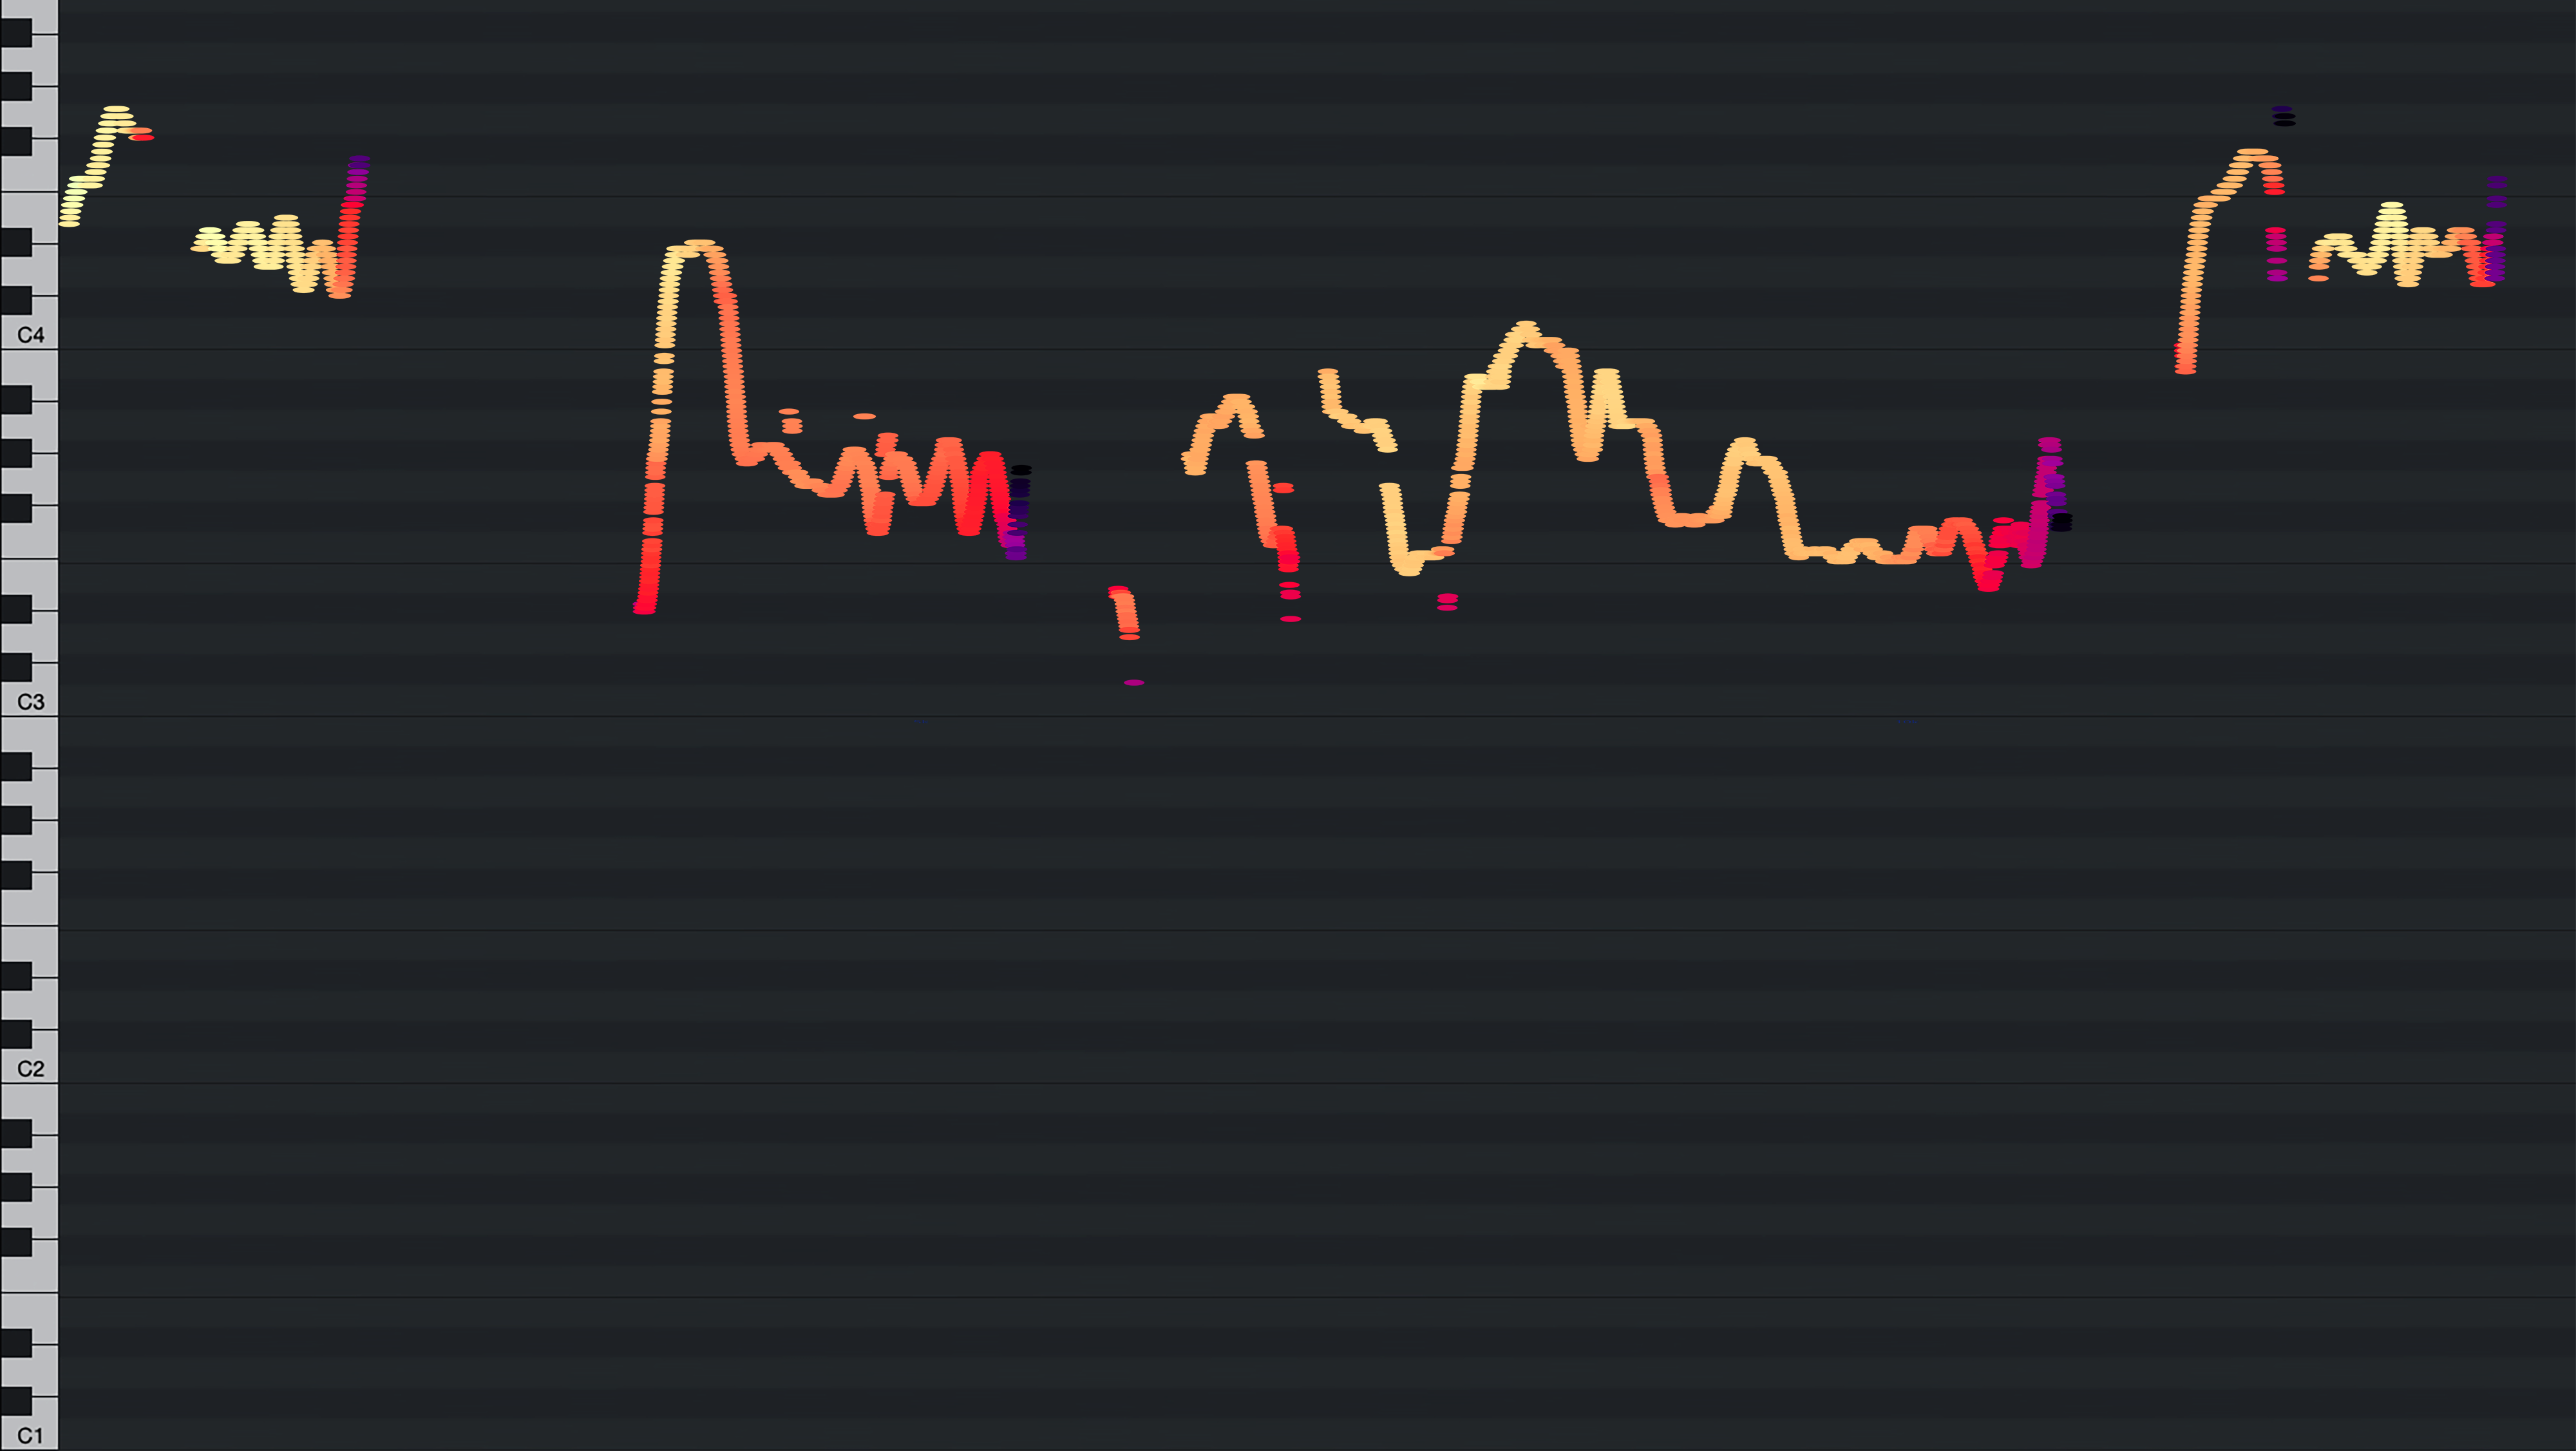
\includegraphics[width=\textwidth]{papers/autotune/images/Pianoscale_Example_Detuned_CMNDF.png}
	\caption{Pitch-Detektion mit CMNDF.}
    \label{autotune:fig:pitchDetektionCMNDF}
\end{figure}


Es zeigt sich, dass kommerzielle Software-Tools mit grosser Wahrscheinlichkeit die CMNDF-Methode verwenden.
So stimmen die eigens mittels CMNDF berechneten Tonhöhen mit denjenigen der kommerziellen Software \textit{Steinberg Cubase 12 Pro VariAudio} überein,
welche als Referenz verwendet wurde. Dies ist dargestellt in Abbildung \ref{autotune:fig:pitchDetektionCMNDFReference}.

\begin{figure}
	\centering
	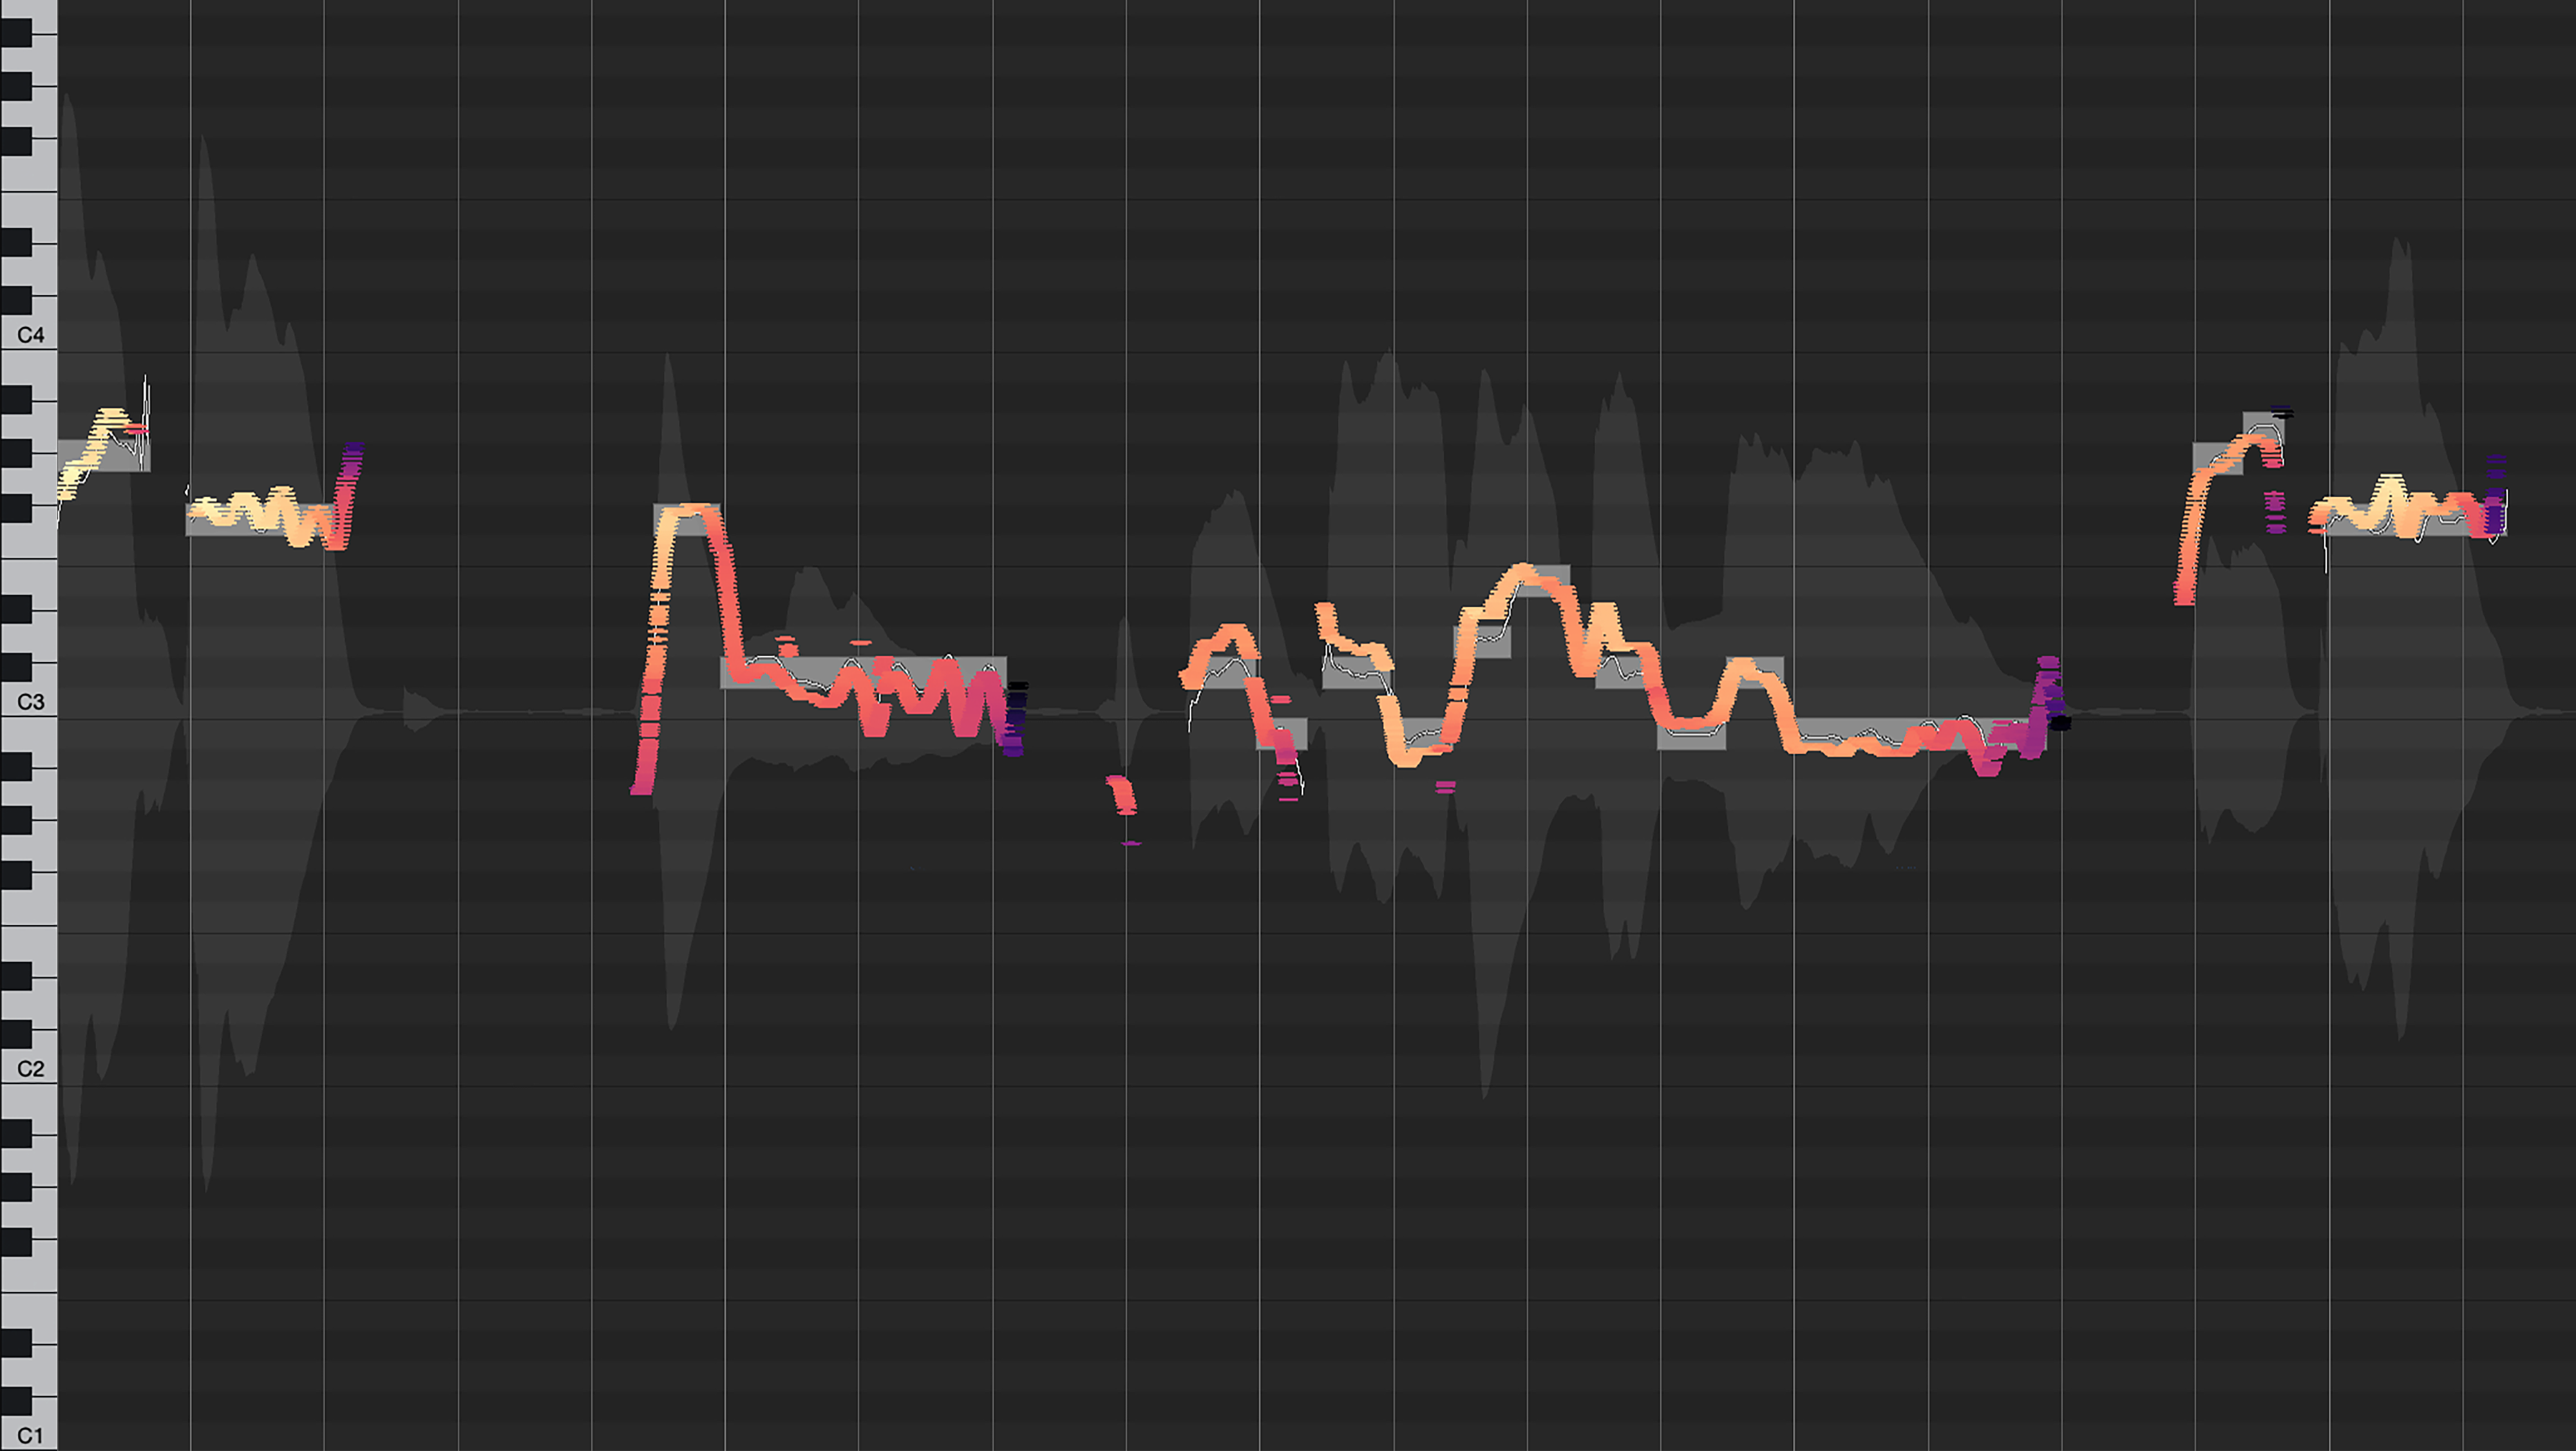
\includegraphics[width=\textwidth]{papers/autotune/images/Pianoscale_Example_Detuned_CMNDF_Reference.png}
	\caption{Vergleich der Tonhöhenbestimmung mit CMNDF und kommerzieller Auto-Tune Software (Steinberg Cubase 12 Pro VariAudio).}
    \label{autotune:fig:pitchDetektionCMNDFReference}
\end{figure}
